\documentclass[tikz,border=5pt]{standalone}
\usepackage{times}
\usepackage{amsmath,amssymb}
\usetikzlibrary{positioning,fit,arrows.meta,backgrounds,shapes.geometric,calc,shadows,decorations.pathreplacing}

\begin{document}
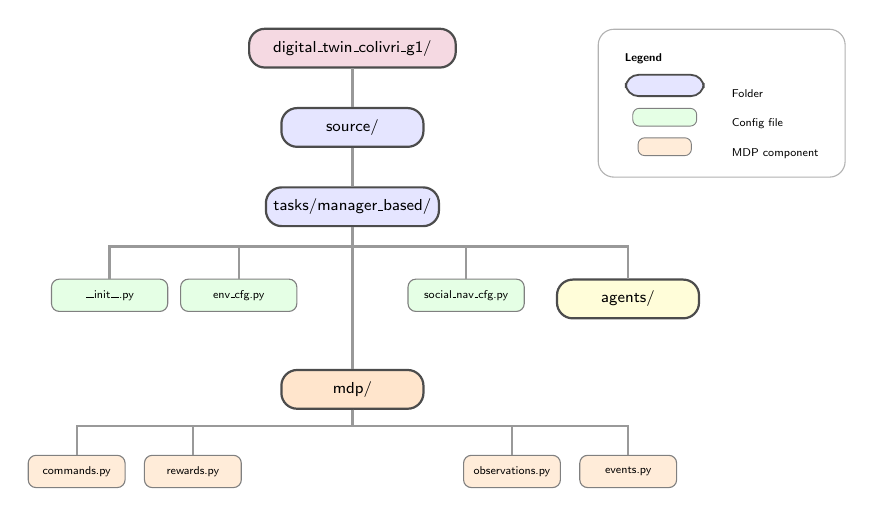
\begin{tikzpicture}[
    scale=0.82,
    transform shape,
    node distance=0.4cm,
    folder/.style={
        draw=black!70,
        rounded corners=2mm,
        minimum width=2.2cm,
        minimum height=0.6cm,
        font=\sffamily\scriptsize,
        fill=blue!10,
        thick,
        align=center
    },
    file/.style={
        draw=black!50,
        rounded corners=1mm,
        minimum width=1.8cm,
        minimum height=0.5cm,
        font=\sffamily\tiny,
        fill=green!10,
        align=center
    },
    mdpfile/.style={
        draw=black!50,
        rounded corners=1mm,
        minimum width=1.5cm,
        minimum height=0.5cm,
        font=\sffamily\tiny,
        fill=orange!15,
        align=center
    },
    arrow/.style={-, thick, color=black!40}
]

% Root
\node[folder, fill=purple!15, minimum width=3.2cm] (root) {digital\_twin\_colivri\_g1/};

% Source level
\node[folder, below=0.6cm of root] (source) {source/};
\draw[arrow] (root.south) -- (source.north);

% Tasks level
\node[folder, below=0.6cm of source] (tasks) {tasks/manager\_based/};
\draw[arrow] (source.south) -- (tasks.north);

% Main files and folders - horizontal spread
\node[file, below left=0.8cm and 1.5cm of tasks] (init) {\_\_init\_\_.py};
\node[file, below left=0.8cm and -0.5cm of tasks] (envcfg) {env\_cfg.py};
\node[file, below right=0.8cm and -0.5cm of tasks] (socialcfg) {social\_nav\_cfg.py};
\node[folder, fill=yellow!15, below right=0.8cm and 1.8cm of tasks] (agents) {agents/};
\node[folder, fill=orange!20, below=2.2cm of tasks] (mdp) {mdp/};

% Connect to tasks
\draw[arrow] (tasks.south) -- ++(0,-0.3) -| (init.north);
\draw[arrow] (tasks.south) -- ++(0,-0.3) -| (envcfg.north);
\draw[arrow] (tasks.south) -- ++(0,-0.3) -| (socialcfg.north);
\draw[arrow] (tasks.south) -- ++(0,-0.3) -| (agents.north);
\draw[arrow] (tasks.south) -- (mdp.north);

% MDP components - spread out more
\node[mdpfile, below left=0.7cm and 2.4cm of mdp] (commands) {commands.py};
\node[mdpfile, below left=0.7cm and 0.6cm of mdp] (rewards) {rewards.py};
\node[mdpfile, below right=0.7cm and 0.6cm of mdp] (obs) {observations.py};
\node[mdpfile, below right=0.7cm and 2.4cm of mdp] (events) {events.py};

% Connect MDP
\draw[arrow] (mdp.south) -- ++(0,-0.25) -| (commands.north);
\draw[arrow] (mdp.south) -- ++(0,-0.25) -| (rewards.north);
\draw[arrow] (mdp.south) -- ++(0,-0.25) -| (obs.north);
\draw[arrow] (mdp.south) -- ++(0,-0.25) -| (events.north);

% Legend - positioned at top right
\node[draw=black!30, rounded corners=2mm, fill=white, inner sep=0.2cm, anchor=north west] at (3.8,0.3) {
    \begin{tabular}{cl}
    \multicolumn{2}{l}{\textbf{\sffamily\tiny Legend}} \\[2pt]
    \tikz\node[folder, scale=0.55] {}; & \sffamily\tiny Folder \\[1pt]
    \tikz\node[file, scale=0.55] {}; & \sffamily\tiny Config file \\[1pt]
    \tikz\node[mdpfile, scale=0.55] {}; & \sffamily\tiny MDP component
    \end{tabular}
};

\end{tikzpicture}
\end{document}
